\chapter*{Appendix A}
\addcontentsline{toc}{chapter}{Appendix A}

\section*{Gantt Chart}

\subsection*{A.1 Project Development Timeline}

The development of the Collective Mobile Journaling Application followed a structured timeline spanning approximately 14 weeks, from early March 2025 to mid-June 2025. The project timeline reflects realistic development patterns with periods of intensive work followed by consolidation phases.

\begin{figure}[H]
\centering
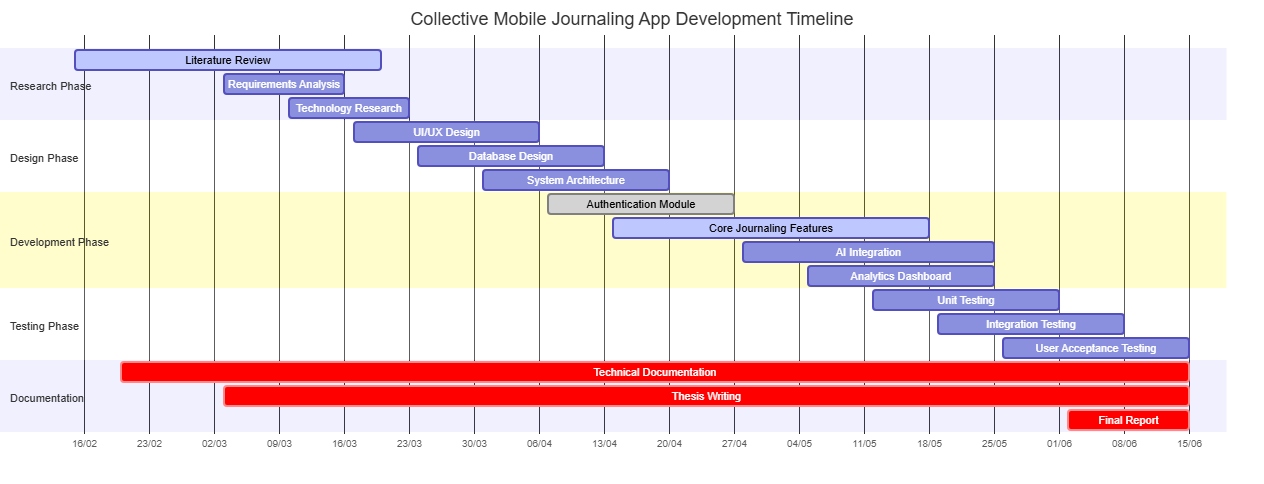
\includegraphics[width=\textwidth]{files/imgs/gantt_chart.png}
\caption{Collective Mobile Journaling App Development Timeline}
\label{fig:gantt-chart}
\end{figure}

The Gantt chart illustrates the overlapping nature of software development phases, showing how research activities began before the official Week 1 start date and continued throughout the project. The timeline demonstrates realistic development patterns including:

\begin{itemize}
    \item \textbf{Extended Research Phase}: Literature review and requirements analysis extended beyond initial estimates to ensure comprehensive understanding
    \item \textbf{Iterative Design Process}: UI/UX design overlapped with development phases, reflecting agile methodology principles
    \item \textbf{Parallel Development}: Core features and AI integration developed concurrently to optimize timeline
    \item \textbf{Continuous Documentation}: Technical documentation and thesis writing maintained throughout the project lifecycle
    \item \textbf{Comprehensive Testing}: Multiple testing phases ensuring quality deliverables
\end{itemize}

The critical path activities (marked in red) include documentation tasks that span the entire project duration, emphasizing the importance of continuous documentation in academic projects.
